% CREATED BY DAVID FRISK, 2016
\chapter{Results}

\epigraph{ \textit{If you can not measure something, you can not improve it.}}{--- \textup{William Thomson Kelvin}}

\section{Evaluation metrics}
Generally speaking in Computer Science, every domain and application could have different evaluation metrics, for example the energy efficient of a CPU is a heavy metrics in embedded systems while in a high performant CPU latency and throughput are dominant metrics. As said that, evaluation metrics strongly depend on the end-users, therefore the designers have to make assumption on the end-user intentions and applications.\\
In this work the assumptions are that the accelerator will be deployed into an embedded system and at the same time it should give to the user a certain degree of flexibility for running Neural Network models. Thus, as it is suggested \cite{paper:1} the following metrics are used:
\begin{itemize}
\item Accuracy, quality of the final result of inference process.
\item Throughput, for measuring real time performance. It depends on the number of internal computation cores.
\item Latency, for interactive applications.
\item Energy and Power, for a mobile device in which there is a limited battery capacity meanwhile for data centers stringent power ceilings due to cooling costs.
\item Hardware cost (Utilization Factor in case of an FPGA) of chip area and process technology.
\end{itemize}
\newpage
\section{Utilization Factor}
An important aspect of an embedded system is the on-die utilization area. Those kinds of system are usually deployed on tightly area constrained chips for hiding their presence to the user.
Therefore, it is important to measure and understand the behavior on the Utilization of the FPGA (used as area measurement in this case) of the design as the size of Matrix Multiplication Unit increases and in parallel the throughput.\\
The Utilization Factor, composed of Look-up-Table, Flip Flops and Digital Signal Processor usage, is expected to increase as the size of Multiplication Matrix increase and the bit width of Computation Unit.

\begin{figure}[!htbp]
\centering
\captionsetup{justification=centering}
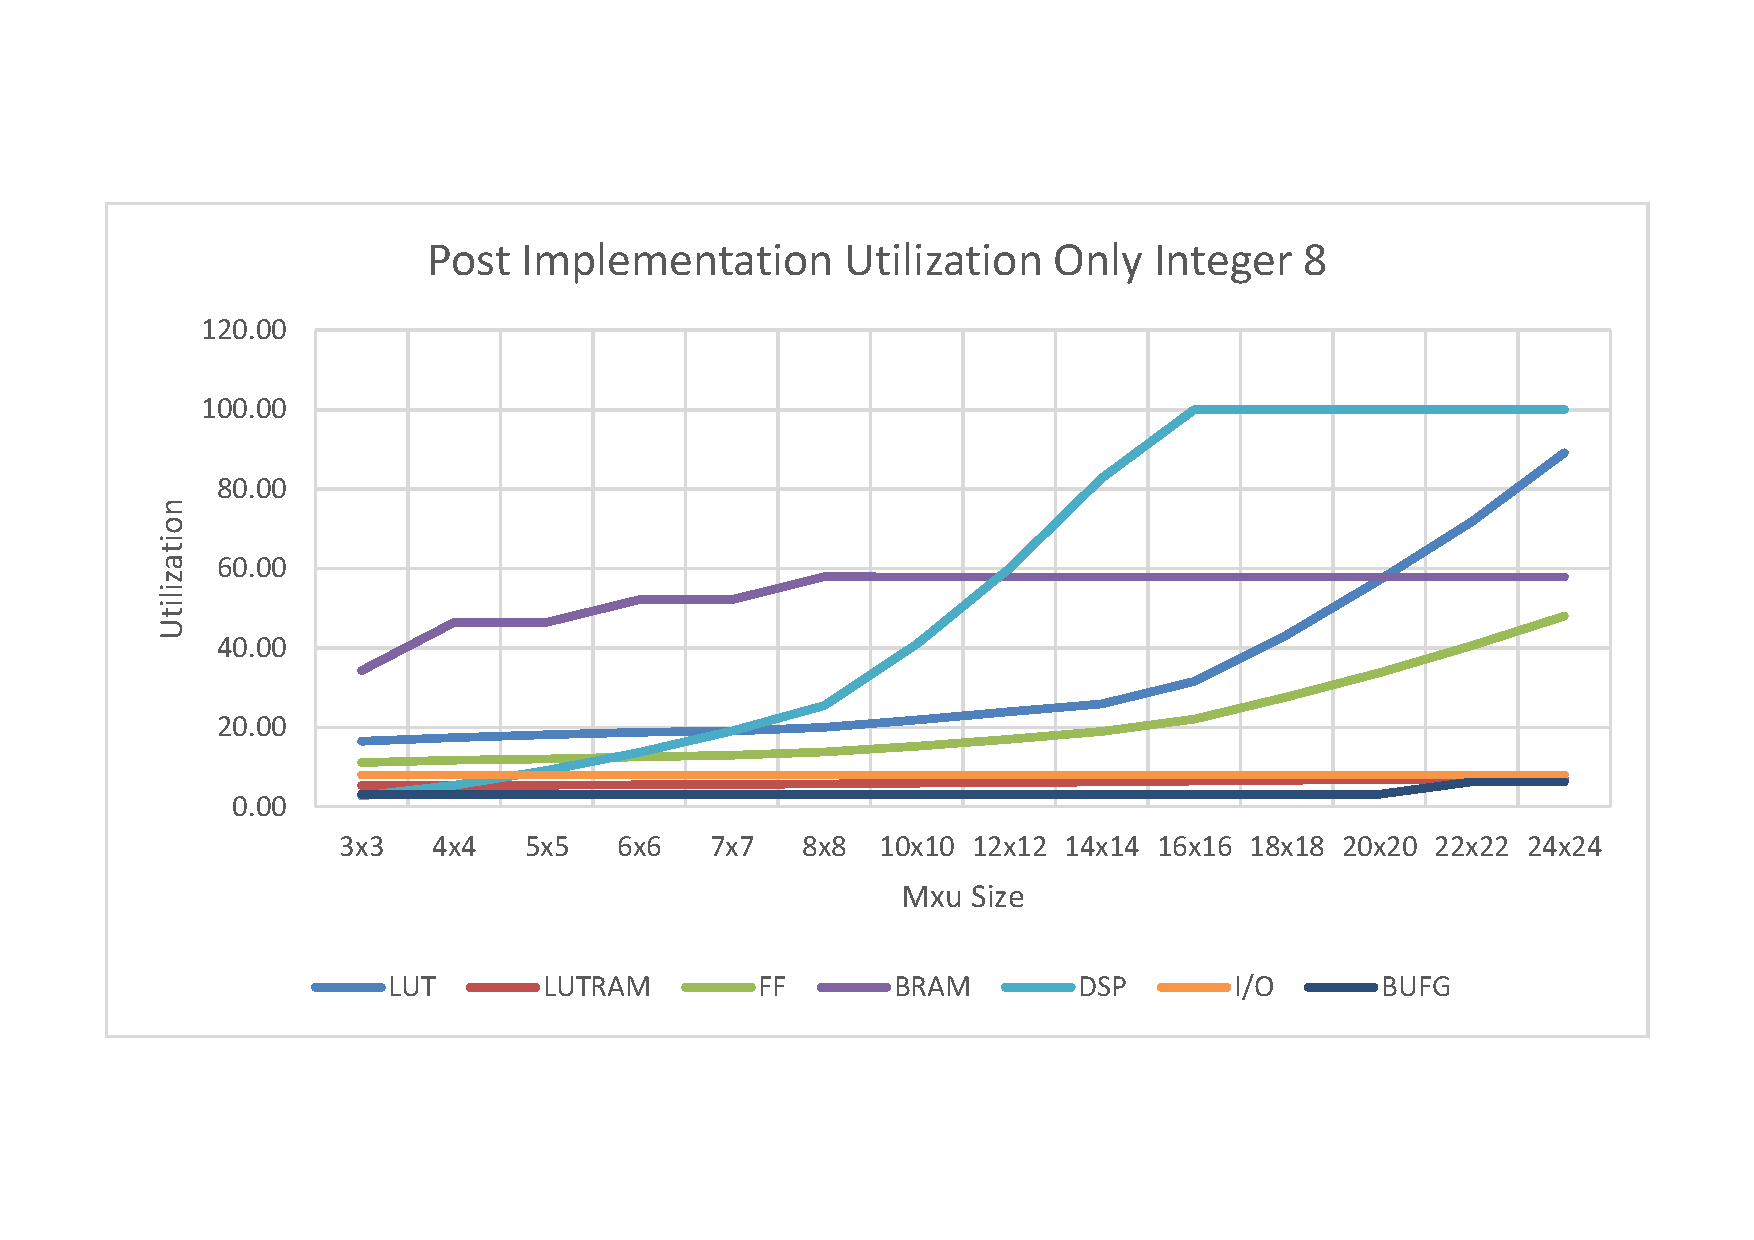
\includegraphics[scale=0.5,angle=0]{./figure/graphs/graph_utilization.pdf}
\label{fig:ut8bit}
\end{figure}


\newpage
\section{Energy and Power Consumption}
\todo[inline]{report power from vivavo}

\begin{figure}[!htbp]
\centering
\captionsetup{justification=centering}
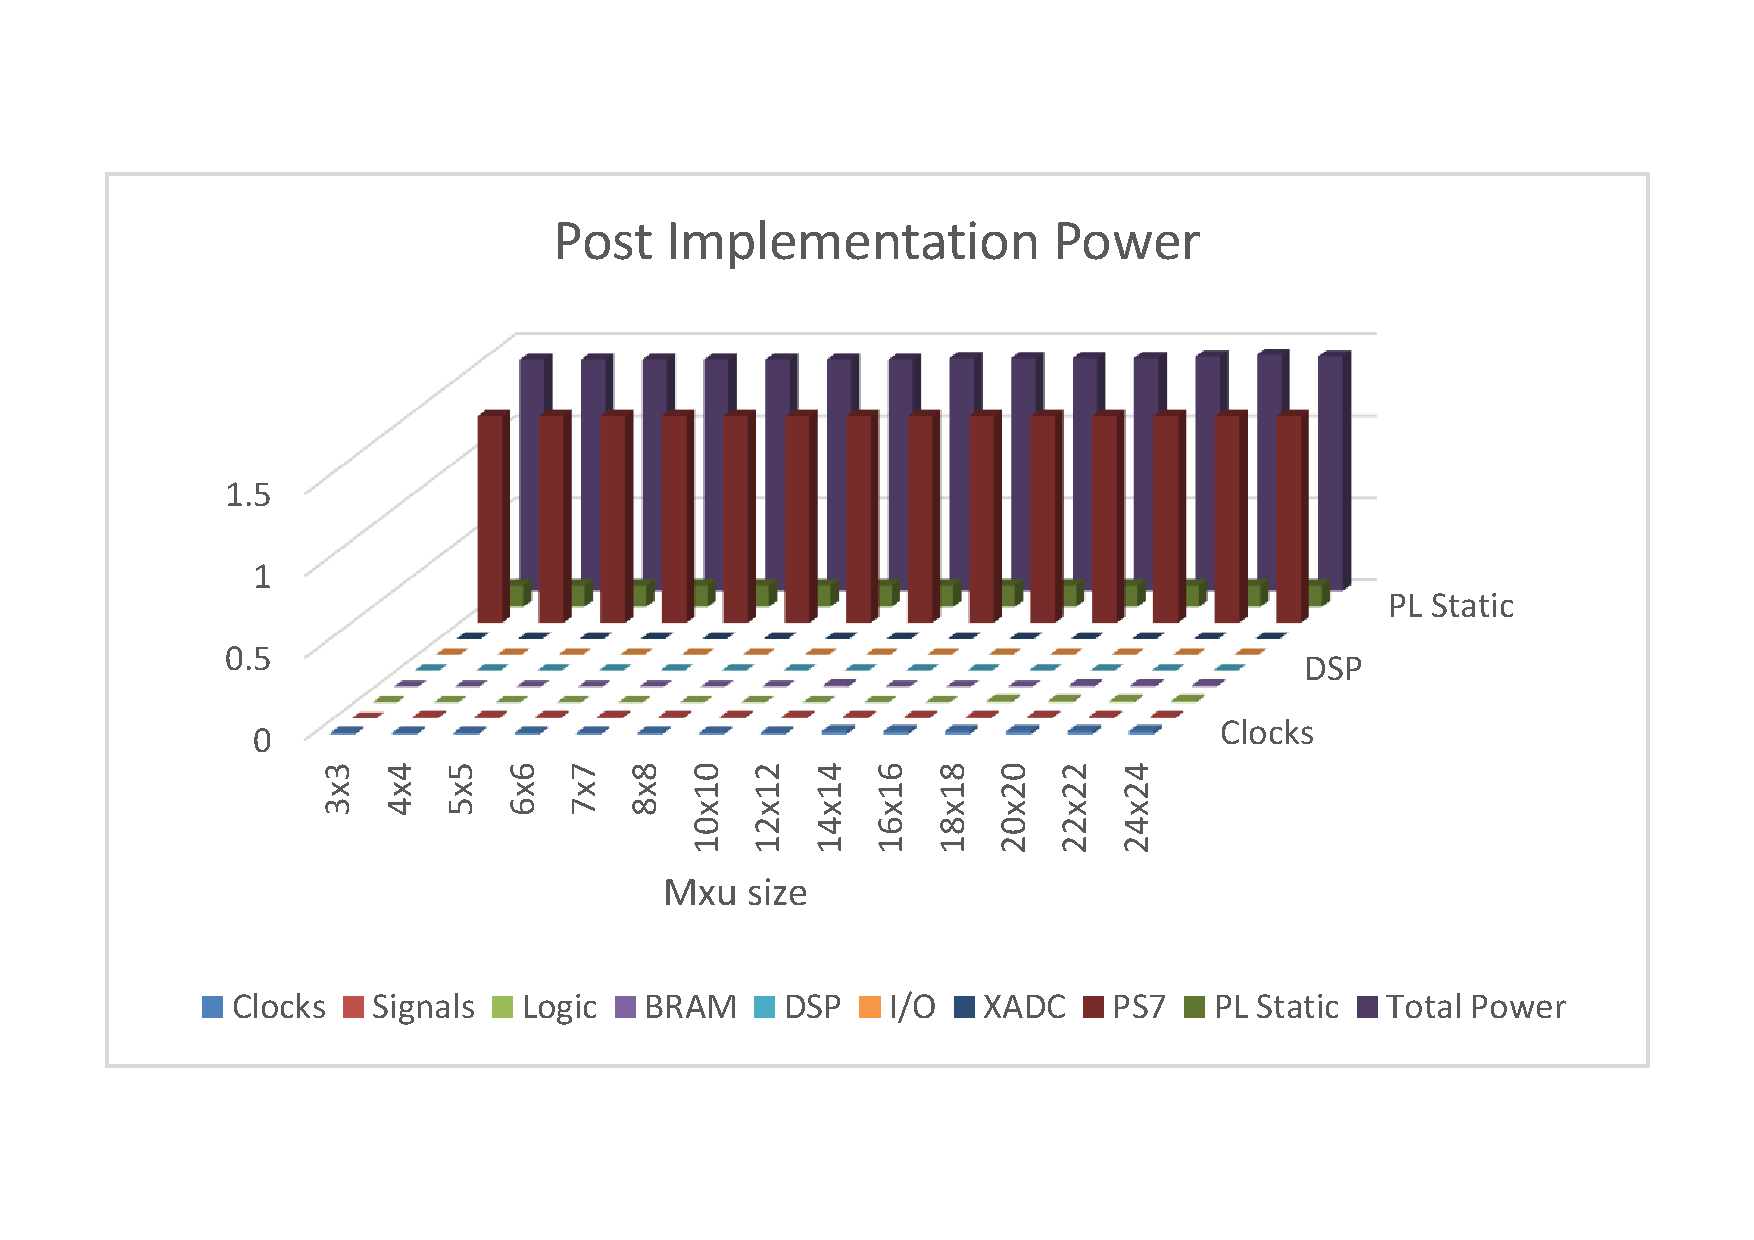
\includegraphics[scale=0.5,angle=0]{./figure/graphs/graph_power.pdf}
\label{fig:pow8bit}
\end{figure}

\newpage
\section{Throughput}
\begin{figure}[!htbp]
\centering
\captionsetup{justification=centering}
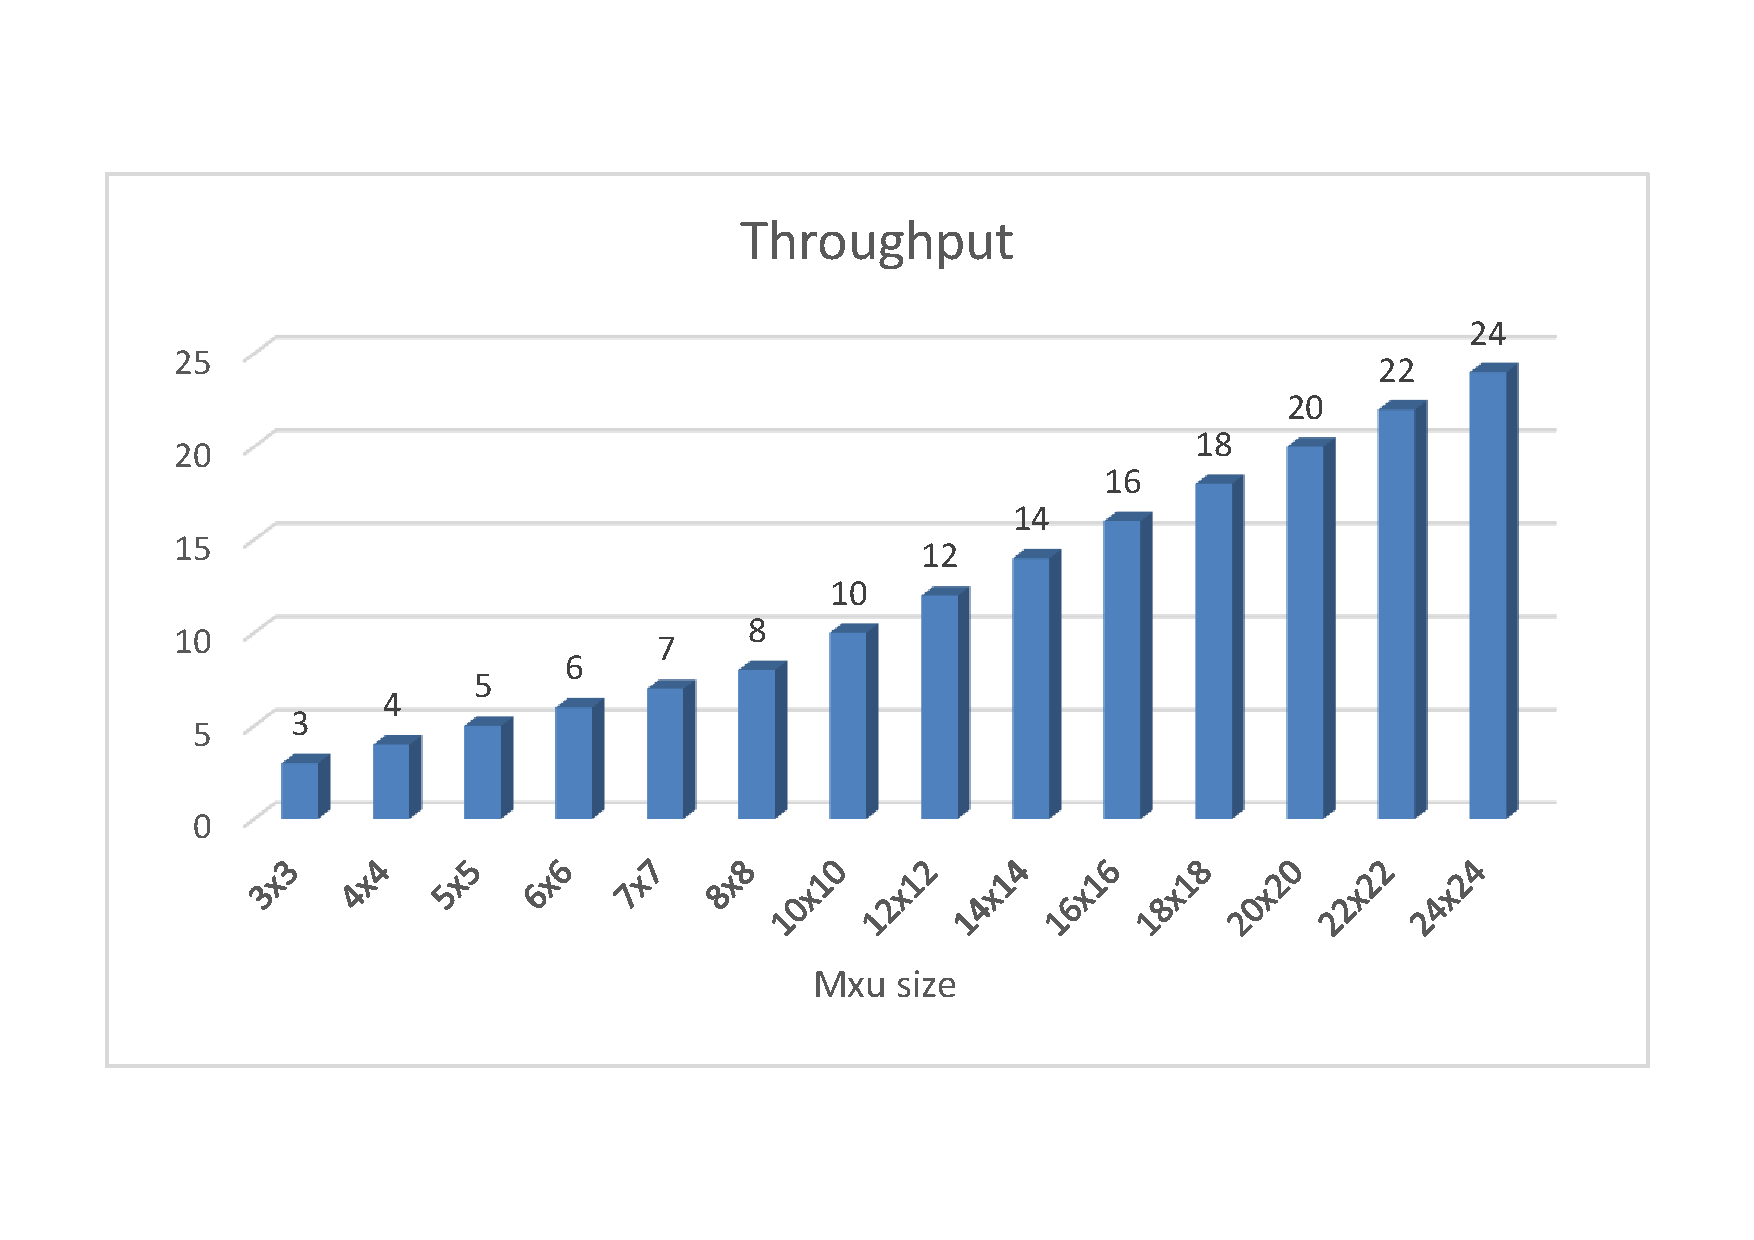
\includegraphics[scale=0.5,angle=0]{./figure/graphs/throughput.pdf}
\label{fig:tp8bit}
\end{figure}

\todo{chart which grows linear with the increase of the mxu size, assumption is that data are provided for each processing element}

\newpage
\section{Latency}

\begin{figure}[!htbp]
\centering
\captionsetup{justification=centering}
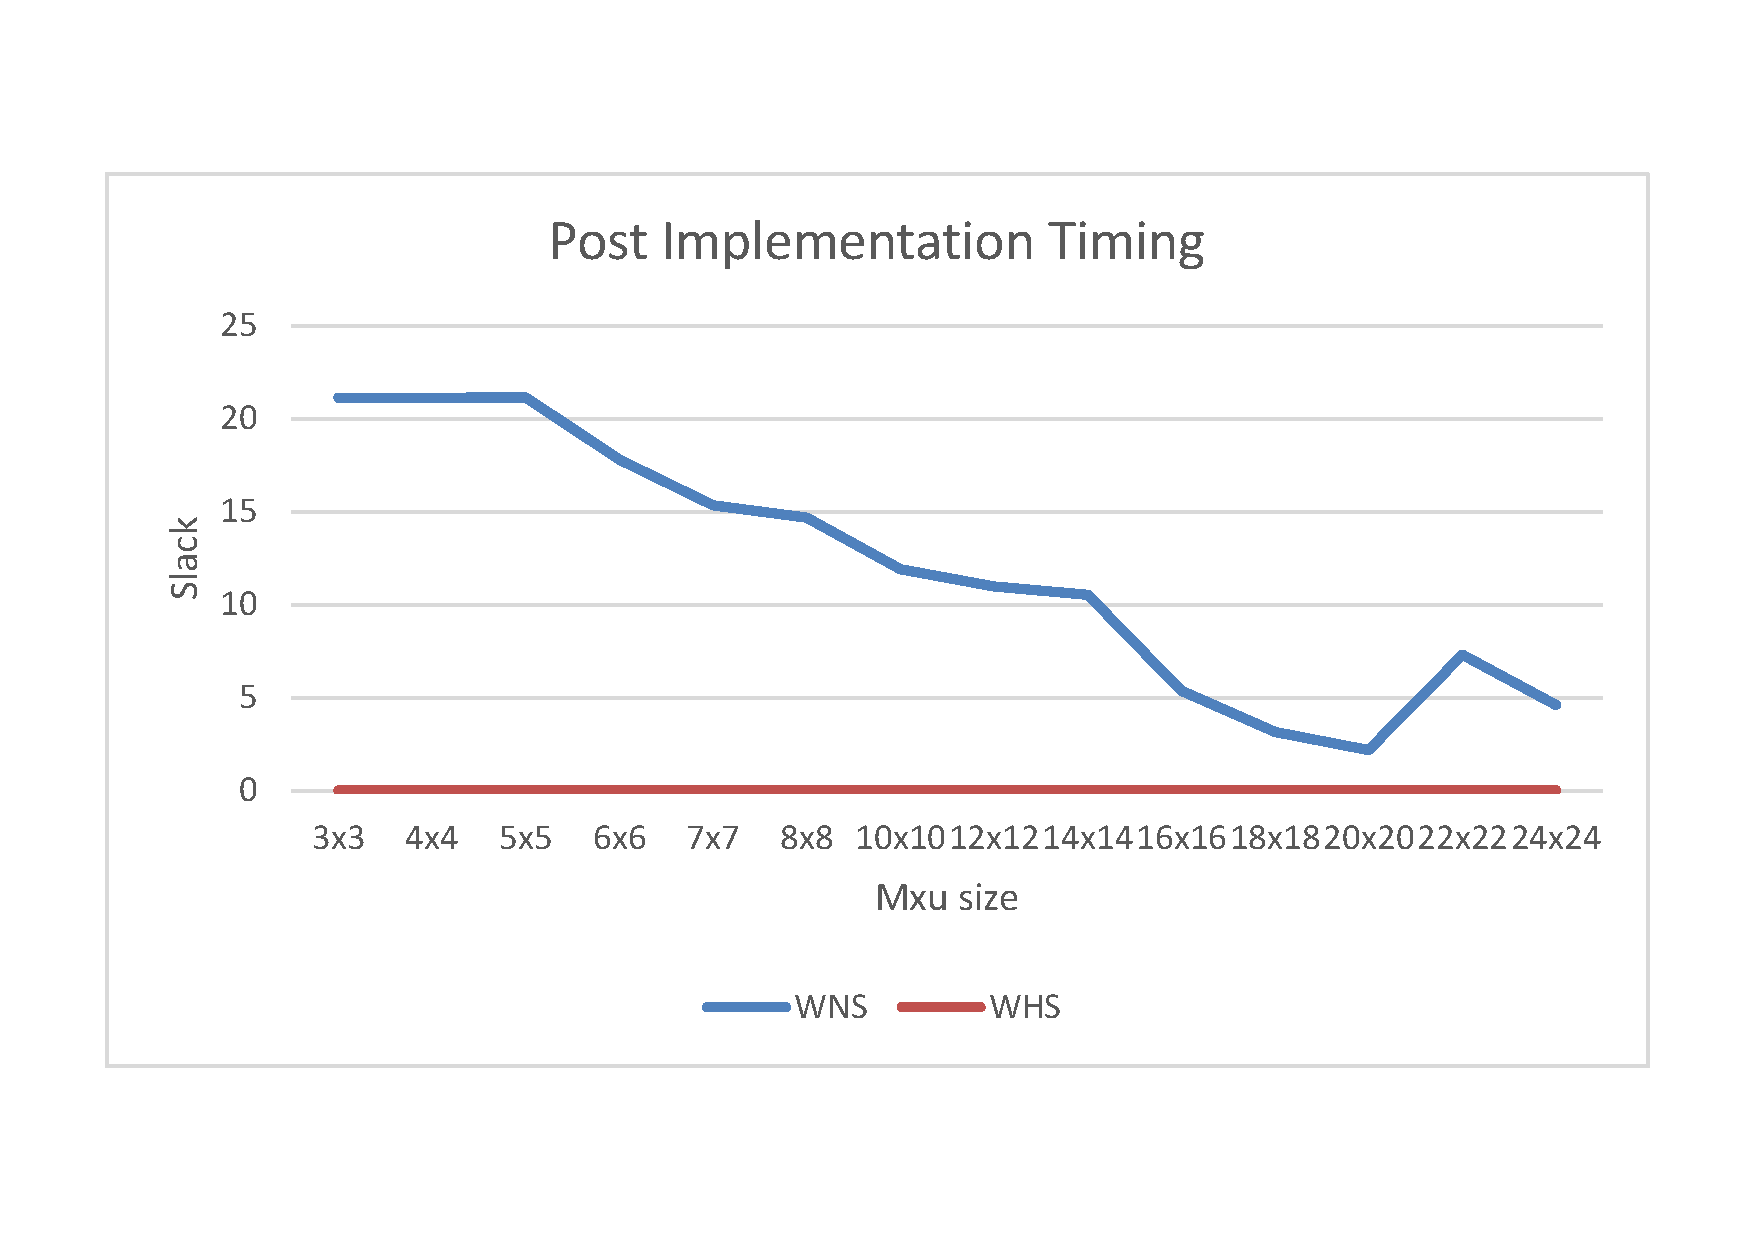
\includegraphics[scale=0.5,angle=0]{./figure/graphs/graph_timing.pdf}
\label{fig:tim8bit}
\end{figure}


\todo[inline]{also chart for the various timing for every size of mxu and different clocks}
\todo[inline]{comparison also with the same NN running on the a gpu+cpu machine, also total time of the execution of entire NN and accelerated part } 

\begin{center}
\begin{table}[!htbp]
\centering
\begin{tabular}{ |p{3cm}||p{2.5cm}|p{2.5cm}|p{2.5cm}|p{2.5cm} }
 \hline
Model & CPU (host) & GPU(host) & CPU(Pynq Z2 board) & CPU(Pynq Z2 board) + accelerator \\
 \hline
 MNIST & & &\\
 Mobile Net V2& & &\\
 Cifar 10& & &\\
 Image Classification& & &\\
 \hline
 \end{tabular}
 \caption{Table to test captions and labels}
\label{table:1}
\end{table}
\end{center}

\newpage
\section{Accuracy}
\todo[inline]{list of NNs with the accuracy of the reference model(the one running on the board's cpu) with the cpu+accelerator run }

\begin{center}
\begin{table}[!htbp]
\centering
\begin{tabular}{ |p{3cm}||p{3cm}|p{3cm}|p{3cm}|  }
 \hline
Model & Reference Output  & Actual Output & Relative Error\\
 \hline
 MNIST & & &\\
 Mobile Net V2& & &\\
 Cifar 10& & &\\
 Image Classification& & &\\
 \hline
 \end{tabular}
 \caption{Table to test captions and labels}
\label{table:2}
\end{table}
\end{center}